\documentclass[dvips,letterpaper,12pt]{report}
\usepackage[square,numbers]{natbib}
\usepackage{url}
\usepackage{thesis}
\usepackage[dvips]{graphicx}
\usepackage{float}
\usepackage{caption}
\usepackage{subcaption}
%\usepackage{svg}
\usepackage{amsmath}
\usepackage{array}
\usepackage{mathtools}
\usepackage{multirow}
\usepackage{makeidx}
\usepackage{longtable}
\usepackage{listings}
\usepackage{color}
\usepackage{alltt}
%\usepackage{epstopdf}
%\numberwithin{equation}{section}

%\definecolor{dkgreen}{rgb}{0,0.6,0}
%\definecolor{gray}{rgb}{0.5,0.5,0.5}
%\definecolor{mauve}{rgb}{0.58,0,0.82}

\lstset{frame=tb,
  language=Java,
  aboveskip=3mm,
  belowskip=3mm,
  showstringspaces=false,
  columns=flexible,
  basicstyle={\small\ttfamily},
  numbers=none,
  numberstyle=\tiny\color{gray},
  keywordstyle=\color{blue},
  commentstyle=\color{dkgreen},
  stringstyle=\color{mauve},
  breaklines=true,
  breakatwhitespace=true
  tabsize=3
}
%\makeindex
\begin{document}

\pagenumbering{roman}

\thesistitle
	{A New Approach for Evaluation of Stereo Correspondence Solutions in Outdoor Applications of Augmented Reality}
	{Baharehsadat Pourazar}
	{Master of Sciences}
	{Department of Computer Science}
	{April 2014}

%\addcontentsline{toc}{chapter}{Abstract}
\begin{center}
\textbf{\large Abstract}
\end{center}
For many years, researchers have made great contributions in the fields of augmented reality (AR) and stereo vision. 
One of the most studied aspects of stereo vision since the 1980s has been \textit{Stereo Correspondence}, which is the problem of 
finding the corresponding pixels in stereo images, and therefore, building a disparity map.
As a result, many methods have been proposed and implemented in order to properly address this problem. 
Due to the emergence of different techniques to solve the problem of stereo correspondence, having an evaluation scheme to assess 
these solutions is essential. Over the past few years, different evaluation schemes have been proposed 
by researchers in the field to provide a testbed for assessment of the solutions based on specific criteria.
For instance, the Middlebury Stereo and the Kitti Stereo benchmarks
are two of the most popular and widely used evaluation systems through which a solution can be evaluated and compared 
to others. 
However, both of these models take a general approach towards evaluating the methods, that is, they 
have not been designed with an eye to the particular target application.
In our proposed approach, steps are taken towards an evaluation design based on the potential applications of stereo methods.
Considering the target application while evaluating the methods enables us to better define the criteria for \textit{efficiency}, that is, the processing time, 
and the required \textit{accuracy} of the disparity results.
Since AR has attracted more attention in the past few years, 
the evaluation scheme proposed in this research is designed based on outdoor AR applications which can take advantage of
stereo vision techniques to obtain a depth map of the surrounding environment. This map can then be used to
integrate virtual objects in the scene that respect the occlusion effects that are expected to occur based on the depth of the real objects. 


%\addcontentsline{toc}{chapter}{Acknowledgements}
\begin{center}
\textbf{\large Acknowledgements}
\end{center}

\vspace{1cm}

Foremost, I would like to express my sincere gratitude to my supervisor, Dr. Oscar Meruvia-Pastor, for his continuous support, motivation, insightful advice and 
kind guidance throughout my research program. This 
thesis would have not been possible without the generous resources provided by him, the Department of Computer Science, and Memorial University.

I would like to express my heartfelt appreciation to Dr. Sam Bromley for his patience, constant encouragement, and insightful, challenging comments which compelled me to always
do better.

I am deeply grateful to my family who never stopped supporting me throughout all my studies, even when we were far from each other. I would have never been the person I am today if 
it was not for their unconditional support.

Last but not the least, I want to thank my fellow labmates in Computer Vision Lab for the interesting ideas we shared, for all the sleepless nights we spent together before deadlines, 
and for all the fun we had together in the last two years. Studying in Memorial University along with my peers in the department has been a great experience for me
and is absolutely an unforgettable memory.

\include{contents}
\include{figures}


\pagenumbering{arabic}
\chapter{Introduction}
\label{chap:Introduction}

Augmented reality (AR) systems combine standard video inputs with computer-generated objects and
usually provide real-time interaction for the users. 
In general, an augmented reality system can be defined with the following properties \cite{azuma01} :
\begin{itemize}
\item Combination of real and virtual environment
\item Registration (alignment) of real and virtual objects
\item Real-time interaction
\end{itemize}
This concept was pioneered in the 1960s by an American computer scientist named Ivan Sutherland
who created the first head-mounted augmented reality
system with the help of one of his students \cite{azuma01}.

Combining virtual objects and annotations with real
world scenes has proved to be an effective way of conveying information about the surrounding environment to
the user and can be useful in many applications such as gaming, medical surgeries, tourism, and other entertaining, informative or instructional tasks.

Many mobile augmented reality systems have been built over the past decades, from the Touring Machine in 1997 by Feiner et al. \cite{fei97} 
to Google AR glasses which was announced in 2013 \cite{google}; however, most of these prototypes have remained experimental
due to certain difficulties and constraints of using them in practical applications \cite{dras96,liv05}. To name two of the most important constraints
we can refer to:
\begin{enumerate}
\item Human factors in augmented reality 
\item High demand of computational resources in order to provide a real-time interaction between the user and the system
\end{enumerate}

%\section{Obtaining Depth Cues in AR Systems}
\section{Image Registration in Augmented Reality}
AR systems overlay 2D or 3D virtual objects on real scenes. Therefore, depending on the application, certain accuracy is required for 
registration of the virtual and real objects in the scene, for which certain knowledge of the location of the user and different objects 
is essential \cite{azuma01}.
In an AR system, different techniques can be used to 
obtain the user's location and the position of other objects in the environment. In many AR systems, fiducial markers are used
in the environment with computer vision tracking methods to find the actual position of the objects within the scene. This method, however, is 
more useful in prepared, indoor AR environments. Tracking sensors such as gyroscope and accelerometer along with video sensors can 
also be used as complementary techniques to provide information on the user's position and viewing orientation \cite{azuma01}. 
%however, they usually rely on known features in the surrounding environment.
However, for unprepared, outdoor environments, especially in mobile AR applications, it is not practical to use markers in various locations 
in the scene, 
and therefore, a markerless technique, such as obtaining a dense depth map of the surrounding environment,
must be considered as an alternative to find the position of the objects in the scene.
To obtain the depth of the 
surrounding environment several depth sensing technologies can be used such as 3D laser scanner, depth cameras or regular cameras. However, in order to have a mobile AR
system that is easy to carry around, the weight of the whole system will be more of a concern, hence, 
3D laser scanners and depth cameras are not proper choices for such systems.
Depth cameras, such as Kinect, or DS325 have a strong limitation in the viewing range; Kinect, 0.8m to 4m \cite{mkinect}; and DS325, 0.15m to 1m \cite{skinetic}. 
On the other hand, 3D laser scanners can
generate very accurate depth maps; however, they are normally expensive and their price ranges from \$3,000 to \$300,000 or more, 
depending on their accuracy and range.
Therefore, among all these technologies, using several 
cameras to generate a depth map of the surrounding environment seems to be a more practical approach for outdoor mobile augmented reality systems. {\newline}
However, using several cameras to get the depth map of the scene requires certain conditions to be met, geometrically and computationally. Many researchers have already looked into
this particular problem, i.e, finding the 3D position of the points in the scene from two or multiple views using regular cameras \cite{sze11}. Attempts of these researchers have resulted in
certain techniques in computer vision to find the depth of different points in an environment using one or more stereo pairs taken from slightly different points of view of the same scene.
These techniques are known as {\it Stereo Correspondence} or {\it Stereo Matching} in computer vision \cite{sze11}. Stereo matching has been one of the most studied subjects in computer vision for 
many years now and there are many solutions proposed by researchers to address this problem using different techniques; however, finding the corresponding pixels in stereo pairs with certain level of 
accuracy and in real-time for practical applications still remains a challenging task. {\newline}

% Motivation - Objective - Contributions %
\section {Motivation}

Due to the emergence of different techniques to solve the problem of stereo correspondence, having an evaluation scheme to assess 
these solutions is essential. Over the past few years, different evaluation schemes have been proposed 
by researchers in the field to provide a testbed for assessment of the solutions based on specific criteria.
For instance, the Middlebury Stereo \cite{mideval} and the Kitti Stereo benchmarks \cite{kitti}
are two of the most popular and widely used evaluation systems through which a solution can be evaluated and compared 
to others. 
However, both of these models take a general approach towards evaluating the methods, that is, they 
have not been designed with an eye to the particular target application. In other words, 
they mainly focus on the fundamental aspects of designing a stereo algorithm as a solution per se to generally
find the \textit{best matches} of corresponding pixels in stereo pairs. 

In this study, we take steps towards an evaluation design which is based on the potential 
applications of stereo vision methods.
This enables us to better define and adjust the criteria for \textit{efficiency} and 
\textit{the best correspondence matches} while doing the evaluation.
Since AR has attracted more attention in the past few years, 
the evaluation scheme proposed in this study is designed based on outdoor AR applications which take advantage of
stereo vision techniques to obtain a depth map of the surrounding environment. This map will then be used to
integrate virtual objects in the scene that respect the occlusion property and the depth of the real objects in the scene. 

In other words, our motivation in this research is to study the possibility of combining stereo vision approaches with 
AR systems considering the most important constraints that AR systems
normally encounter in outdoor environments. 
In fact, our fundamental research question is: \newline

\begin{quote}
\textbf{``Can the combination of stereo matching techniques with augmented reality meet the requirements of an AR system in outdoor 
environments?''} \newline
\end{quote}

In order to find the answer to this question, some other questions are raised:
\begin{quote}
\textbf {``How does the human visual system (HVS) perceive depth?''}\newline
\textbf {``What is the standard angular disparity for the human visual system and how would it affect an AR system?''} \newline
\textbf {``How can we evaluate stereo vision in an augmented reality framework and what are the important factors we need to consider for 
	this type of evaluation?''} \newline
\textbf {``In a combination of augmented reality with stereo vision, what is considered an \textbf{\textit {accurate}} depth result?''} \newline
\textbf {``How can a three dimensional model be built from stereo images using computer vision techniques?''}\newline
\textbf {``What are the requirements to maintain an interactive augmented reality application for the user?''} \newline
\end{quote}

To answer these questions, we have designed and implemented a testbed for evaluation of
the stereo matching solutions based on specific criteria which will be thoroughly described in the following chapters.

As a starting point for our AR system, the depth map generated from two or multiple camera views
will be used as the depth source to determine the position of the objects in the scene when
overlaying virtual objects at different locations and depth levels in the real environment. 
For our research, we decided to narrow down our study to the effect of using stereo vision techniques
on two of the most important constraints of an AR system mentioned earlier in this chapter: 
{\it human factors} and {\it real-time interaction}. {\newline}
Human perception of depth can vary depending on the environment and under different circumstances. Many studies have focused on the evaluation of human perception of depth within different frameworks
and in different applications, such as virtual reality and augmented reality, which have recently 
attracted more attention \cite{wann95,dras96,liv05,jer05,swa07,kru10}.
These studies show that the viewer perception of depth
is inversely proportional to his/her distance from the object \cite{kru10,swa07,jer05,liv05}. For instance, in \cite{swa07} some experiments are designed to study and evaluate human
perception of distance, which is the absolute depth of the objects from the observer, for an outdoor augmented reality application in urban settings. 
However, in this research we are more interested in the human perception of relative depth in stereo vision, which is the ability to perceive and distinguish 
the depth of different objects relative to each other. 
In binocular vision, the minimum depth difference between two points 
that can be detected in the visual system is known as {\it Stereoscopic Acuity} or {\it Stereoacuity} \cite{pfa2000}. More detail about
this metric will be provided in the following chapters.
We have investigated the standard stereoacuity in the human visual system and applied it to our evaluation in order to obtain the smallest detectable depth of 
objects in human binocular vision based on their distance from the observer.

Providing real-time interaction in an AR system for the user requires the processing time and update rate of the whole system to keep up ideally with the standard video frame rate, 
between 24fps and 
30fps, or higher. 
However, studies show that in practice to build a reasonable interactive augmented world the processing rate should not be less than half of the video frame rate \cite{hertz00}. 
There are different approaches to speed up a system: 
\begin{enumerate}
\item Using more advanced technology and hardware
\item Achieving a more sophisticated and efficient software design
\end{enumerate}
However, having access to advanced technology and hardware is not always feasible and even the most advanced 
technologies have some limitation in their memory space and computational capability
which may not meet the requirement for some real-time applications. 
Therefore, we have decided to focus more on the second approach while designing our evaluation system which also looks into one of the
key properties of an AR system mentioned earlier, that is, the real-time user interaction.

One of the most important features that makes our evaluation unique and different from the others is that we have 
designed the evaluation process of the stereo matching solutions with an eye to augmented 
reality applications in outdoor environments.
In order to address the speed factor, we evaluate the results based on the requirements of providing an interactive AR system for the user.
In addition, to address the constraint of computational resource, we have integrated a module in our design that 
focus on the evaluation of particular regions in the scene rather than 
the whole image. 
It is known that distinctive features such as {\it edges}, either in RGB or depth images from a scene, 
play an important role in many computer vision applications, such as object detection and 
tracking, determination of a set of reliable correspondences to build a 
3D model that helps with better perception of object locations in 3D space \cite{mart01,sze11}.

Therefore, in an augmented reality application, wrong depth results, especially in those regions, 
which will lead to erroneous registration of virtual and real objects, 
can be perceived easier by the human visual system. This can lead to poor performance of the system and possibly faulty interaction between 
the user and the augmented world.
Figure \ref{fig:ARreg} shows an accurate and faulty registration of objects in a 3D environment that results from an accurate and 
wrong disparity map in the areas of depth discontinuities.

\begin{figure}[H]
\centering
\subcaptionbox{Accurate registration of objects}
[.5\linewidth]{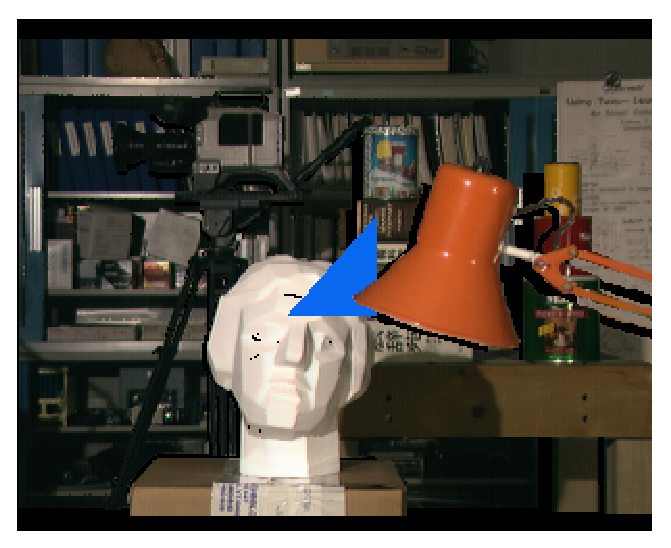
\includegraphics[scale=0.7]{tsukuba}}%
\subcaptionbox{Erroneous registration of objects}
[.5\linewidth]{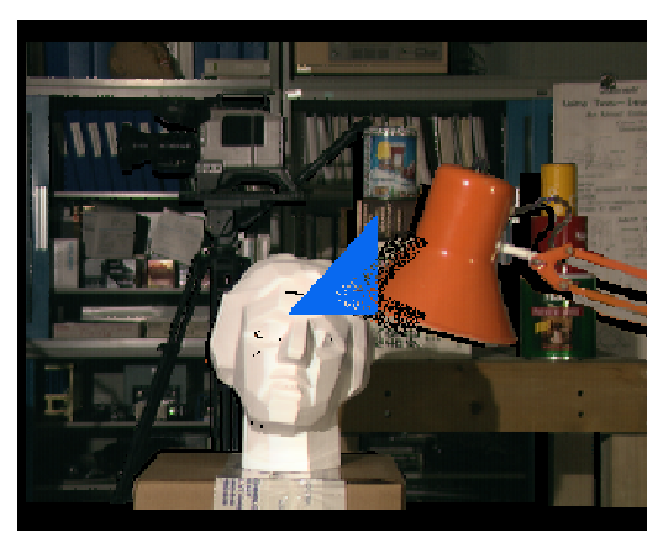
\includegraphics[scale=0.7]{tsukubadist}}%
\caption{Integration of objects in a 3D environment}
\label{fig:ARreg}
\end{figure}

Therefore, we focus the evaluation in our model
on the depth edges in the scene and their surrounding regions \cite{liv05,kru10}.
Our hypothesis is that salient edges caused by depth discontinuities, which can also represent the object boundaries and occlusion, and their surroundings
are one of the most important depth cues for the observer 
to perceive the depth of different objects in the scene \cite{sze11}. 
Furthermore, the regions of depth discontinuity and occlusion are known as two of the most challenging parts in the image
for the stereo correspondence algorithms \cite{sch02}.
Finding correct depth values in these 
regions can lead to a higher quality combination of the virtual and real objects in the scene, thus providing a more reasonable augmented world 
for the user to interact with.

%%Is this part needed to be in this chapter?%%

\section{Methodology}
To achieve our objectives in this research, we have surveyed some of the existing approaches to solve the problem 
of stereo correspondence and the geometrical principles of the 3D reconstruction from stereo pairs, which will be explained more 
in the next chapters. 
In order to investigate the benefits of our proposed model, we have evaluated two sample stereo matching algorithms in our system. 
These algorithms are:
\begin{enumerate}
\item Semi-global block matching, also known as SGBM, which is a modified version of the semi-global matching by Hirschmuller \cite{hir08}.
\item The solution  proposed by Mei et al., ``On building an accurate stereo matching system on graphics hardware'' \cite{mei11}, also known as ADCensus.
\end{enumerate}

SGBM is now integrated in the Open Source Computer Vision Library (OpenCV) \cite{sgbm}, and therefore, we have used this implementation
in our evaluation.
On the other hand, since no implementation of ADCensus is available in the public vision libraries, we have used our own implementation of it.
Although ADCensus is originally proposed as a GPU-based solution, we have used the CPU implementation of it in our evaluation.

SGBM is selected as it has shown to generate acceptable results within 1-2 seconds on the typical test images \cite{hir08}; moreover,
its integration within the OpenCV library has made its usage more common in different applications. 
ADCensus is also currently ranked as one of the best solutions 
for solving the problem of stereo correspondence in terms of general accuracy, regardless of the running time, 
according to the Middlebury evaluation table \cite{mideval}.
In addition, AdCensus does not currently exist in the KITTI evaluation table which motivates us to evaluate its performance
under real world circumstances with outdoor stereo images.

\section{Organization of Thesis}
This report is organized in the following structure.
We discuss a background of the related work and concepts in Chapter 2 where the geometry of stereo vision, 
stereo correspondence problem, and a survey of the stereo solutions will be reviewed. 
Moreover, we will introduce some of the key computer vision techniques employed
during this research work. Chapter 3 introduces some of the most relevant concepts in binocular vision to this study.
In Chapter 4, we will explain our system and its design and components in detail. Chapter 5 discusses the experiments
conducted for the evaluation of the proposed system in the framework of an outdoor AR application.
In Chapter 6, we discuss the shortcomings and benefits of our system based on the results from Chapter 5. 
Consequently, a discussion of the potential aspects for improvement 
and future research will also be provided.


\chapter{Background and Related Works}
\label{chap:Background}

Stereo vision is the concept of viewing a scene (object) in the real world from slightly different
viewpoints at the same time which results in stereo image pairs. Using computer vision techniques, it is possible to extract depth information from stereo
images. This process is called {\it Stereo Matching} or {\it Stereo Correspondence} in computer vision,
which in fact leads to the construction of a
3D model of a scene from two or multiple views by finding corresponding pixels and therefore, their spatial movement within various views of the same scene \cite{sze11}.

Corresponding pixels in stereo images are the ones that represent the same point in the real
world. As it will be seen shortly in more detail, the amount of horizontal motion of such pixels
in stereo pairs, which is referred to as {\it disparity}, is inversely proportional to the
distance from the observer, i.e., depth; however,  estimation of the exact depth of the points requires some
other information as well, such as the position, and the calibration data of the cameras that took the pictures.
While the physical and geometrical approaches to this problem are well understood by researchers in the field, the process of finding the corresponding pixels correctly, yet efficiently
and measuring the disparity to generate a dense depth map still remains a challenging task. \newline

\section{Epipolar Geometry}
Understanding the fundamentals in the underlying geometry of stereo matching helps to better understand the principal idea behind all the methods designed to address this problem, 
thus facilitating the comprehension of 3D model reconstruction from stereo image pairs. Therefore, we will thoroughly describe the basic geometry of stereo matching in this section. \newline
If we consider two cameras that are looking at a particular scene from slightly different view points, a back projection of any point in the 3D space via rays passing through each camera centre
would result in two distinct points on each image plane. For simplicity, we will refer to the point in space as $P$, and its projection on the first (left) and second (right) image planes,
as $P^{'}$ and ${P}^{"}$ respectively. \newline
As a result of $P$'s back projection on the image planes, an important property will emerge between the points and the camera centres, which is coplanarity of all these points. 
This plane, also referred to as {\it epipolar plane}, passes through $P^{'}$, $P^{"}$ and the camera centres, thus intersecting each image plane. 
It should be noted that this property, from which the consequent properties are derived, is the building block of stereo matching methods. 
Let us denote the specified plane by $S$ for further reference. 
Since $S$ passes through the camera centres, it clearly traverses the line 
that connects two camera centres. This line, which is known as the {\it baseline}, intersects each image plane at a point called the {\it epipole}; denoted by ${e}^{'}$ and ${e}^{"}$
in Figure \ref{fig:epg}. 
Consequently, the intersection of the plane $S$ and each of the image planes, creates a line called {\it epipolar line} \cite{hart2000}. 
The {\it epipolar line} always passes through the {\it epipole} in the image plane. 
These concepts, illustrated in Figure \ref{fig:epg}, constitute the important components of the stereo correspondence geometry.

\begin{figure}[!h]
\centering
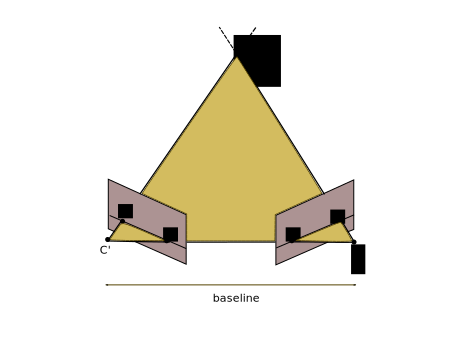
\includegraphics[width=0.5\textwidth]{epipole}
%\includesvg{epipole}
\caption{Epipolar geometry}
\label{fig:epg}
\end{figure} 

Now, we can define the problem of stereo correspondence as a case in which the location of $P^{'}$ in the image plane is known, while the
corresponding point $P^{"}$ is unknown; therefore, the problem can be stated as an attempt to find the correspondence of $P^{'}$ in the second image plane. Based on the aforementioned 
properties, we know that $P^{"}$ is located somewhere on the line, the epipolar line,
created by the intersection of the plane traversing the ray that goes through $P^{'}$ and the first camera centre and the {\it baseline}. This line is in fact, the projection of the ray going
through $P^{'}$ and the first camera centre, on the right image plane. Therefore, the search for the corresponding point, $P^{"}$, will be limited to merely scanning the corresponding 
epipolar line on the second image plane rather than the whole image.

%\begin{figure}{h!}
%\centering
%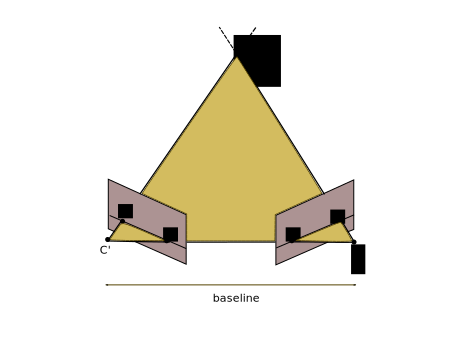
\includegraphics[width=1.5in,height=1.5in]{epipole}
%\end{figure}

It is now apparent that in order to find the correspondence of a particular point $P^{'}$, in the second image plane
the corresponding epipolar line, must first be sought. 
The projection from a point to its corresponding epipolar line can be obtained through certain transformations in space; normally a rotation and translation, Figure \ref{fig:rectify}.
For further geometrical calculations, these transformations can be represented
with a matrix that is only dependant on the camera's properties, not the scene \cite{hart2000}.
However, dealing with these transformations while looking for the corresponding points, can increase the complexity of stereo matching algorithms to certain levels \cite{sze11}; therefore, 
in order to avoid this issue, many stereo matching approaches are proposed based on the assumption that image pairs are first warped \cite{sze11}.
This process is known as {\it image rectification} which is basically achieved by first having the cameras rotated in a way that their optical axis, 
the line passing through the camera centre which is perpendicular to the image plane, are parallel to each other; 
i.e. their optical axis is perpendicular to the baseline. As a result of this transformation, the epipoles are sent to infinity. 
Furthermore, it might be necessary to have the cameras tilted so that their {\it y} axis also becomes perpendicular to the optical axis. 
After these two steps, corresponding epipolar lines actually becomes horizontal scanlines; Figure \ref{fig:rectify}. This pre-processing step significantly constrains the process of searching 
for corresponding points and eliminates certain complications in stereo matching algorithms \cite{sze11}.

\begin{figure}[!h]
\centering
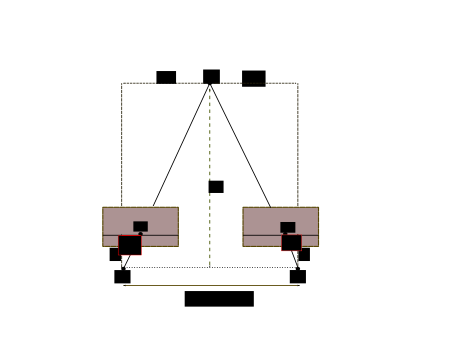
\includegraphics[width=0.65\textwidth,trim=22mm 0mm 0mm 150mm,clip]{rectdisp}
\caption{Rectified image pairs and disparity geometry}
\label{fig:rectify}
\end{figure} 


Using the rectification model and epipolar geometry described earlier, 
derivation of the geometrical relation through which the depth of a certain point in 3D space 
can be obtained, will be straightforward. This relation is presented as follows \cite{sze11}:
\begin{align}
X_{L}/Z=x_{l}/f \\
-X_{r}/Z=-x_{r}/f  \Rightarrow B-X_{L}/Z=-x_{r}/f \\
\intertext{By adding these two equations:} \Longrightarrow  B/Z=(x_{l}-x_{r})/f\\
\text{if} && x_{l}-x_{r}=d \Rightarrow d=Bf/Z
\end{align}
where f is the {\it focal length} measured in pixels, B is the {\it baseline}, Z is the {\it 3D depths}, and d is {\it disparity}. The relationship between corresponding pixels in the left
and right images according to disparity {\it d} is also as follows:
\begin{align}
{P}^{"}_{x}={P}^{'}_{x}+d(x,y) \\
{P}^{"}_{y} = {P}^{'}_{y}
\end{align}
Therefore, based on the aforementioned formulas, the depth of points in 3D space can be easily calculated after finding the corresponding pixels in multiple views and consequently their
disparities \cite{bol87,oku93,sch02}.

\section{Stereo Correspondence Algorithms}
A survey of the field shows that the algorithms which address stereo correspondence problem can be roughly divided into two main classes \cite{sch02}. These classifications are commonly known as:
\begin{enumerate}
\item Sparse Correspondence Algorithms
\item Dense Correspondence Algorithms 
\end{enumerate}

In this section, we are going to briefly describe the important specifications of the algorithms belonging to each of these two categories.
\subsection{Sparse Correspondence Algorithms}
Sparse correspondence algorithms, also known as feature-based algorithms, are the early stereo matching methods. In the 1980s, this class of algorithms received considerable attention by
many researchers in computer vision \cite{dhon89}.
In this type of methods, particular features in an image, such as edges, 
points, line segments, or other distinctive features are extracted; therefore, the search for corresponding pixels is only applied to these regions. 
Consequently, algorithms of this
sort result in a sparse disparity map \cite{matt89,hsie92, sze11}. The introduction of feature-based algorithms has mainly been motivated by three important factors \cite{bro03,sze11}:
\begin{itemize}
\item Lack of advanced hardware and technology for exhaustive computational tasks 
\item Constraint of the search area in order to find more reliable matches.
\item Image pairs with different illumination, where edges or some other particular features preserve their photometric properties, and therefore, are the only regions reliable enough to 
be used for correspondence search.

However, the requirement of having dense depth maps for many applications and also the emergence of efficient {\it dense correspondence algorithms}, have diverted the attention away
from this class of algorithms in the last 20 years.
\end{itemize}

\subsection{Dense Correspondence Algorithms}
Unlike feature-based methods, dense correspondence algorithms try to find the
correspondences for all the pixels in the image, and therefore, result in a dense disparity map. Most recent algorithms and studies have focused on this class of algorithms since many applications 
nowadays, such as graphical rendering, 3D model construction, or augmented reality require a dense depth map of the scene. 
However, these algorithms face many challenges that need to be properly
addressed, such as finding the depth values in occluded regions, depth discontinuities, and textureless areas \cite{sch02,bro03}.

Dense correspondence algorithms are usually classified in two groups based on how they assign
disparities to pixels \cite{sze11}:
\begin{enumerate}
\item Local approaches
\item Global approaches
\end{enumerate}

\subsubsection{Local Approaches} 

Local methods tend to find the disparity of each pixel based on its neighboring pixels. In
other words, the disparity of a pixel is calculated in a finite window containing its neighboring pixels, based on a particular metric, e.g. the intensity values \cite{sch02}.

These methods make an implicit smoothness assumption for the pixels in the search
window, and therefore, assign the same disparity to all the pixels belonging to the same window which could result in incorrect disparity values in slanted surfaces or
depth discontinuities \cite{hirsch02}. This assumption can be considered as one of the major drawbacks of local methods.
Another drawback of local methods is their dependency on the window size \cite{sch02}. A fixed window size can raise certain problems in these algorithms:
\begin{enumerate}
\item If too large of a window size is considered, due to aforementioned smoothness assumption, the algorithm may result in blurry object boundaries and inaccuracy near depth discontinuities.
\item If the selected window size is too small, the disparity values will be less accurate since little information has been considered for 
finding the correspondences of pixels in the image.
\end{enumerate}

However, a significant advantage of using local approaches is their high speed in finding disparity results.\newline

\subsubsection{Global Approaches}
Unlike local approaches, in global methods the disparity of a pixel depends on the information in
the whole image. Global methods usually include an optimization step of a global energy
function\cite{roy98,bobi99,boyk01,hong10}. In this class of algorithms, an optimal disparity value for each pixel is sought that leads to minimization of a global cost
function that normally combines a data term with an explicit smoothness assumption.

\begin{equation}
E(d)=E_{data}(d)+\lambda E_{smooth}(d)
\end{equation}
The term $E_{data}$ is normally defined as the difference of a common metric, e.g. the photometric property, between the corresponding pixels and is denoted as follows:

\begin{equation}
E_{data}(d) = \sum_{(x,y)}C(x,y,d(x,y))
\end{equation}

where C is a matching cost. The matching cost function can have various definitions depending on the algorithm; however, as mentioned above, it is normally defined as sum of absolute difference 
between the intensity of the corresponding pixels in two images \cite{sch02}.

The term, $E_{smooth}$, is the smoothness assumption based on which the disparity values in different regions are refined. The definition of this term can also vary in 
different solutions. $\lambda$ is also a weighting factor, by which the effect of the smoothness assumption in the global function can be controlled in the algorithm \cite{sze11}.
In order to find the minimum of the global function, certain approaches in computer science have proved to be particularly useful. 
To name some of these approaches, we can refer to dynamic programming, graph cut, and belief propagation. Many researchers have studied and addressed the problem of stereo matching
by applying one of these approaches \cite{sch02,boy01,boy04,kim05,sun11}.

The major drawback of global approaches is normally their high usage of computational resources and low speed. However, 
they usually result in more accurate disparity values \cite{hirsch02,sze11}. 

It is also worthwhile to mention that in the past twelve years, another group of algorithms have emerged which cannot be explicitly classified in any of the previously mentioned groups.
These methods, which are known as {\it Segmentation-based techniques}, first segment the image into regions and then, rather than searching for correspondences per pixel,
they attempt to find the corresponding disparity for each region. A more detailed review of these methods can be found in chapter 11 of \cite{sze11}.

\subsection{Edge Detection}

As mentioned earlier in the "Introduction", salient {\it edges} in the scene are one of the important features 
that can be used in many applications, such as object detection, image stitching, or 3D model reconstruction \cite{sze11}.
Due to their importance in defining the object boundaries and also their role in occlusion occurrence and depth discontinuities in stereo vision, we have also focused on studying them in our
evaluation approach; therefore, we have masked our input data based on the detected edges in the scene. 
In order to extract edges in the image, we have used 
specific algorithms. In this section, we will describe how it is possible to find the most salient edges in the scene using vision techniques.

When looking at a scene, an edge is defined whenever the visual system can perceive a distinguishable variation in color, intensity or texture between 
different regions. \cite{sze11}.
Therefore, a reasonable mathematical approach to detect the edges in an image would be calculating the gradient of the intensity image. However, since an image normally contains a certain amount of
noise which intensifies at higher frequencies, taking the derivatives of the image can lead to significant noise amplification, as it makes high frequency signals more prominent to others.
Therefore, it is better to attenuate high frequencies prior to applying any edge detection approach. 
There are a variety of filters for image smoothing (blurring); however, since we want to attenuate high frequencies, it is better to use a low-pass filter which only passes low frequencies.
A widely known class of image blurring filters in computer vision, are called {\it linear filters}. In linear filtering operators, for each pixel a weighted summation of its neighboring pixels
is used in order to estimate its final value \cite{sze11}. In mathematics, this process can be modelled by convolution of the input signal with a particular function, known as kernel. 
\begin{equation}
g(i,j) = g(i,j)=\sum_{k,l}f(i+k,j+l)h(k,l)
\end{equation}
which is equivalent to:
\begin{equation}
g=f\bigotimes h
\end{equation}
where $f$ and $g$ are the input and output signals respectively, and $h$ is the kernel function which can vary depending on the type of filter. 

Therefore, each filter can modify the input signal differently based on its corresponding kernel function.
Gaussian filter is a filter commonly used for attenuating higher frequencies in an image and filtering out the noise. Since edges in an image may be oriented along any arbitrary direction, 
applying a filter which is biased towards a particular direction in filtering out the noise, will not be a prudent decision. Instead, a better choice would be choosing a filter 
with a symmetric 2D kernel function. 
This feature is particularly found in Gaussian filter, since it employs a 2D symmetric kernel. Because of this unique feature, 
Gaussian filter is normally used in most edge detection algorithms as a pre-processing step.
An isotropic, i.e. circularly symmetric, Gaussian kernel has the following form \cite{sze11}:
\begin{equation}
G(x,y)=\frac{1}{2\pi \sigma ^{2}} e^{-\frac{x^{2}+y^{2}}{2\sigma^{2}}}
\end{equation}
where $\sigma$ is the width of the kernel. 
A more thorough description of Gaussian and some other types of filters can be found in chapter 3 of \cite{sze11}.

After smoothing the image with Gaussian filter, the gradient of the smoothed image should be taken in order to detect the edges. This can be done by convolving 
the signal with a pair of convolution masks in each direction in order to detect the edges, both horizontally and vertically. An edge extracting operator called {\it Sobel} is normally used
for this purpose \cite{sze11}. 
Sobel convolution kernels for both x and y directions are defined as follows \cite{sze11}:

\begin{align}
G_{x} = \begin{bmatrix}
-1 & 0 & +1 \\ 
-2 & 0 & +2 \\ 
-1 & 0 & +1
\end{bmatrix} \\
G_{y} = \begin{bmatrix}
-1 & -2 & -1 \\ 
0 & 0 & 0 \\ 
+1 & +2 & +1
\end{bmatrix}
\end{align}

Following the estimation of image gradients in each direction, the magnitude and the direction of an edge element can then be found by \cite{sze11}:
\begin{align}
G=\sqrt{G_{x}^{2} + G_{y}^{2}} \\
\theta = \arctan (\frac{G_{y}}{G_{x}})
\end{align}

The process of applying Sobel operator masks to the smoothed image, is in fact equivalent to getting the first or second order directional derivative of the smoothed image 
and then look for zero crossings, i.e. where the sign of
the function changes \cite{sze11}. As a result of this process, edge elements are detected throughout the image.
After finding the edge points, it is desirable to have them linked to form continuous contours. Since adjacent edge elements are connected to each other, this can be easily achieved by linking
a detected edge element with its neighbors in both direction \cite{sze11}. As a result, a continuous chain of edges can be detected in the image.
{\it Canny} edge detector, proposed by John F. Canny in 1986 \cite{canny86}, is one of the most commonly used edge detection approaches; however, it should be mentioned that in addition 
to the process described above for detecting the edges in the image, there are also two different thresholds defined 
in this approach that affect the edge linkage step. The purpose of having these two thresholds is elimination of streaks, i.e. certain breakage, that may appear along edge contours. 
By employing these thresholds in the process of edge detection and linkage, any value above the higher threshold will be output as an edge element and when linking the edge element 
to its neighbor to form a continuous contour, only those 
values above the lower threshold will be accepted \cite{canny86}. This process has shown to reduce the streaking effect to a significant amount \cite{canny86}. \newline

\subsection{Morphological Operations}
In addition to linear filters, there is another type of filters known as {\it non-linear filters}. In this type of filtering, unlike linear filters, the final value of a pixel is not necessarily 
a weighted combination of its neighboring pixels \cite{sze11}. 
{\it Median filter, Bilateral filter}, and {\it anisotropic diffusion} are all different types of non-linear filters. Non-linear filters are used for certain image manipulation 
and enhancement tasks, and are commonly used with a particular type of image called {\it binary
image} \cite{sze11}. Binary images, as their name indicates, consist of merely two pixel values, 0 or 1. These images are usually the outcome of filtering the values in an image 
by a certain threshold, thus changing each value to 0 or 1 based on the comparison against the threshold. Binary images are
widely used for {\it masking} operations in image processing \cite{sze11}. Due to extensive application of binary images, certain operations are usually employed to manipulate them. 
These operations are known as {\it morphological operations} \cite{sze11}.
In morphological operations, the original image is convolved with a {\it structuring element}, also known as kernel. 
Structuring element is a mask (i.e. binary image), normally smaller than the original image, 
with which different structures can be defined for later modification of the image. 
{\it Dilation} and {\it Erosion} are two of the most basic and widely used morphological operations in binary image processing.
These two operation are normally used for expansion and erosion of the shapes in the original image. 
In dilation, the structure element which is usually in form of a circle or square with the origin located at its centre, is superimposed on top of the original binary image.
By moving the structure element over the background pixels, each pixel belonging to the background, that 
is overlain by the centre of structuring element, is replaced by foreground value if at least one of the pixels of the structuring element coincide with any pixel marked as foreground.
Erosion, which can be considered as the complementary operation of dilation, follows a similar process, with only the difference that structuring element is moved over foreground pixels and any
foreground pixels will be replaced by background value if at least one pixel of the structuring element overlaps with a pixel marked as background.
Hence, we can state that dilation of the foreground is equivalent to erosion of the background \cite{ritt96}.
\textbf {EXAMPLE IMAGE OF DILATION AND EROSION}

\chapter{Binocular vision and Stereopsis}
\label{chap:BinocularVision}

Binocular Vision is a term used for the visual system of animals with two eyes \cite{how95}, and therefore, applies to human visual system as well. 
Possessing binocular vision not only lead to a better perception of depth
of the surrounding environment, but also help to better perform many visual tasks such as reading, object detection, interaction with surrounding objects such as grabbing and other manipulative 
tasks. However, the most significant advantage of possessing binocular vision is its influence on how the 3D environment, i.e. the depth of surrounding objects relative to each other, 
is perceived by the two eyes. This visual perception of depth in binocular vision is referred to as {\it Stereoscopic Vision}.
In the visual system, depth perception is a phenomenon that normally occurs though different types of cues and information existing in the surrounding environment. 
These pieces of information, known as {\it depth cues} in stereo vision, can be either monocular or binocular depth cues \cite{how95}.
To name a few instances of monocular depth cues, we can refer to motion parallax, lighting and shading, and apparent size. 
However, as previously mentioned, binocular cues which can only be perceived
by stereo vision, play a major role in the perception of depth. One of the most important binocular cues is {\it binocular disparity}, or {\it binocular parallax}. 
It should be noted that the effect of binocular parallax and motion parallax on depth perception are very similar to each other. 
In motion parallax, which is a monocular depth cue, the scene is viewed at different times by the observer moving from side to side, 
whereas in binocular parallax, the scene is viewed from slightly different viewpoints at
the same time by the two eyes, while the observer standing at a fixed position \cite{how95}. \textbf{FIGURE to show this}

\begin{figure}[!h]
\centering
\subcaptionbox{Motion Parallax}
[.4\linewidth]{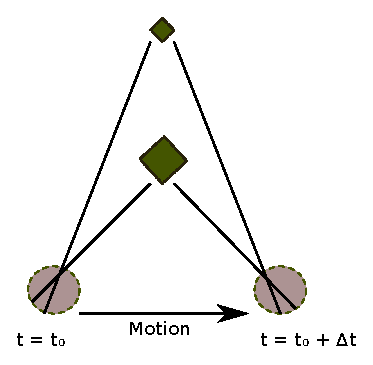
\includegraphics{Mparallax}}%
\subcaptionbox{Binocular Parallax}
[.4\linewidth]{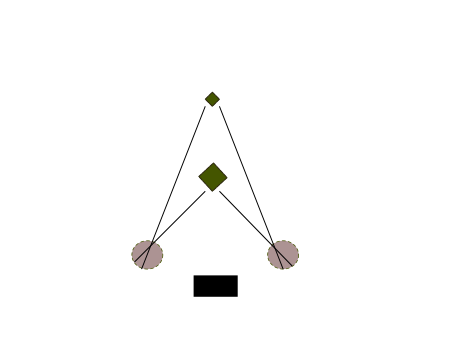
\includegraphics{Bparallax}}%
\caption{Motion parallax and binocular arallax difference}
\label{fig:parallax}
\end{figure}

%\begin{figure}[!h]
%\centering
%\begin{subfigure}[b]{7cm}            
%\frame{\includesvg[width=\textwidth]{Bparallax}}
%\caption{Interpolation for Data 1}
%\label{Fig:bp}
%\end{subfigure}
%
%\hspace{1cm}
%
%\begin{subfigure}[b]{7cm}
%\centering
%\frame{\includesvg[width=\textwidth]{Mparallax}}
%\caption{Interpolation for Data 2}
%\label{fig:mparallax}
%\end{subfigure}
%\caption{blah blah}\label{fig:bpmp}
%\end{figure}

Binocular disparity, which in fact arises from the spatial difference 
between the images of the same scene in the two eyes, provides a relative perception of depth from the surrounding environment. This perception is known as {\it binocular stereopsis} \cite{how95}. 
Another important binocular depth cue is the eyes {\it vergence}, which is the simultaneous movement of the pupils in opposite directions in order to obtain a single vision of an object with the
two eyes. When focusing on an object, the optical axes of the eyes intersect on the object of interest resulting in an angle called vergence angle. Unlike many animals, human visual system 
is capable of adjusting this angle based on the distance from the object.
In stereo vision, the locus of the points that yields a single vision in the visual system is known as the {\it horopter}, and any point located on the horopter is usually called a 
{\it fixation point} \cite{binr83,how95}.
An important property of an object on the horopter is that no spatial difference
exists between the images of the fixated object in the two eyes; i.e. the binocular disparity is zero \cite{how95}. 
Exploiting this property, the disparity of any other object in the scene can be estimated relative to the fixated object by inspecting two important factors: 
whether the object of interest is closer or further than the fixated object and then how much closer or further it is relative to the fixated object.
As a result, the binocular disparity provides a relative perception of depth of the surrounding environment.
In the geometry of stereopsis, the relative disparity between two objects is usually presented as angular disparity in radiant, or seconds of arc.

\section{Stereopsis Geometry and Angular Disparity}

In the following section, we will describe how the angular disparity can be calculated utilizing the geometry of stereopsis \cite{binr83}.

\begin{figure}[!h]
\centering
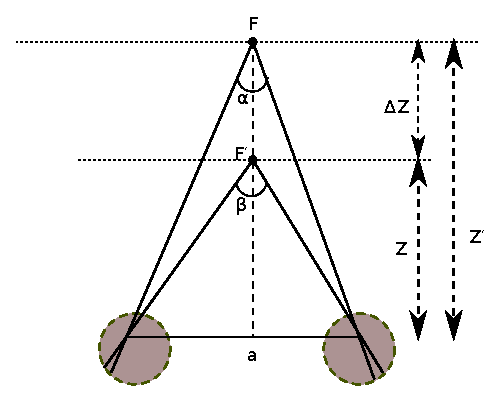
\includegraphics[width=0.5\textwidth]{binocular}
\caption{Binocular disparity}
\label{fig:stereopsis}
\end{figure} 

According to Figure \ref{fig:stereopsis}, we have:
\begin{align}
\theta = \beta - \alpha\\
\alpha = a/Z^{'}\\
\beta = a/Z\\
Z = Z^{'} + \Delta Z\\
\Rightarrow \theta = a/Z - a/Z^{'} = a/Z - a/(Z+\Delta Z) \\
\Rightarrow \theta = aZ+a\Delta Z-aZ/Z(Z+\Delta Z) = a\Delta Z/Z^{2} 
\end{align}

However, when $\Delta Z$ is very small compared to the values of $Z$, the term $\Delta Z$ in denominator can be neglected without significant loss of accuracy. This results in
an approximate formula as follows:

\begin{align}
\label{eq:stac}
\theta = a \Delta Z/Z^{2}
\end{align}

in which $a$ is the distance between the center of the pupils of the two eyes, which is known as interpupillary distance.
It should be noted that this formula estimates the angular disparity in radiant. In order to convert $\theta$ to arcseconds it should be multiplied by:

\begin{align}
180/\pi = 57.296\times360=206.265
\end{align}

Studies show that the visual system capability to distinguish two objects at different distances relative to each other is limited to certain thresholds \cite{binr83,how95}.
This threshold, which is defined as the minimum detectable depth between two 
objects at difference distances, is known as {\it stereoacuity} which varies in different visual systems \cite{binr83,how95}. According to different
experiments \cite{binr83}, the finest detectable angular disparity in human visual system is approximately 10-15 arcseconds. However, a more recent study on
stereoacuity in 60 subjects \cite{garn06} for different age groups, from 17 to 83 using standard stereotests, 
shows that the average stereoacuity for different age groups is as follows:

\begin{minipage}{\linewidth}
\begin{center}
\captionof{table}{Average stereoacuity for subjects of age 17 to 83}
\label{tab:stAcAge}
\begin{tabular}{ |c|c| }
\hline
\textbf{Age Range} & \textbf{Stereo Acuity (arcsecs)} \\ \hline
17-29 & 32 \\  \hline
30-49 & 33.75 \\ \hline
50-69 & 38.75 \\ \hline
70-83 & 112.5 \\ \hline
\end{tabular}
\end{center}
\end{minipage} \newline \newline

Furthermore, studies show that the average interpupillary distance in human is 64mm \cite{how95}. 
Using these values in equation \ref{eq:stac}, the threshold for minimum detectable relative depth 
between two objects can be estimated based on their distance from the observer. \newline 
Studying these concepts and related works in stereo vision, we have designed and implemented our evaluation framework based on standard
stereoacuity measurements mentioned in table \ref{tab:stAcAge}.

\chapter{Design of Evaluation Scheme}
\label{chap:System}

This chapter walks through the steps taken in order to build up our evaluation framework and justification of each decision taken during this design.

%Maybe should be moved to introduction?
\section{Design Criteria}

Since outdoor AR applications are the focus of this study, we have designed our evaluation model within this framework. Moreover, all the evaluation
metrics are measured based on the relevant factors described earlier in chapters \ref{chap:Introduction} and \ref{chap:BinocularVision}.
%Move to Introduction Chapter
%As briefly mentioned in chapter \ref{chap:Introduction}, there are already different evaluation schemes to assess stereo correspondence solutions. The Middlebury Stereo \cite{mideval} and 
%the Kitti Stereo benchmarks \cite{kitti} are two of the most popular and widely used evaluation models through which a solution can be evaluated and compared to others.

%%%
%In these models, a pixel is considered as an \textit{outlier} if the error between the ground truth disparity and the disparity found by the solution is more than 
%a specified pixel threshold in the system, such as 2 or 3 pixels.
%They also provide separate masks for depth discontinuities and occluded regions, in addition to evaluating the whole image.
%%%

%However, both models take a general approach towards evaluating stereo algorithms; that is they have not been designed with an eye to the particular target 
%application.


%In other words, they mainly focus on the fundamental aspects of designing a stereo algorithm as a solution per se to \textit{efficiently}
%find the \textit{best matches} of corresponding pixels in stereo pairs. 
%This perspective may raise some questions for a punctilious researcher, such as:

%\begin{enumerate}
%\item What actually is an \textit{efficient} solution and on what basis is this \textit{efficiency} defined?
%\item What is a \textit{best match} of corresponding pixels and how can it be defined?
%\end{enumerate}


%In fact, these questions have compelled us to study the evaluation of the stereo matching solutions from a different point of view.
%In this design, we take steps towards an evaluation design which is based on the potential applications of stereo methods.
%This enables us to better define and adjust the criteria for \textit{efficiency} and 
%\textit{the best correspondence matches} while doing the evaluation.
%Since AR has attracted more attention in the past few years, 
%the evaluation scheme proposed in this study is designed based on outdoor AR applications which take advantage of
%stereo vision techniques to obtain a depth map of the surrounding environment. This map will then be used to
%integrate virtual objects in the scene that respect the occlusion property and the depth of the real objects in the scene. 
%In other words, the motivation of this research is to study the possibility and usability of integrating stereo vision techniques in an AR system, while considering the most
%important constraints that AR systems normally encounter \cite{liv05}.
%Move to Introduction Chapter

\section{New Evaluation Scheme}

In an augmented reality system, there are certain factors that would affect the functionality and effectiveness of the system \cite{liv05,kru10} and therefore, 
should be carefully considered when designing and evaluating the system. 
These factors may correspond to the surrounding 
environment, technology and hardware constraints, or human factors. 
Figure \ref{fig:AR} illustrates a high level architecture of an AR system with its key components and their related attributes.
\textbf{(FIG of AR) - draw components and mention some of their related factors}

In this study, we have mainly focused on the human factors in AR which were described in chapter \ref{chap:BinocularVision},
and the requirement of having a real-time interactive AR system from the user point of view.

%Concentrating on the requirements of providing a real-time interaction between an AR system and the users, along with
%certain human factors that would affect the functionality of the system,
%has revealed the necessity of involving them in the evaluation of the stereo correspondence methods. Therefore, in order to 
%determine whether a stereo correspondence algorithm can meet the requirements of an AR application, we need an evaluation scheme which can properly assess 
%the \textit{efficiency} of the algorithm and the accuracy of its disparity results based on specific human factors in binocular vision and augmented reality.
%These factors are in fact the concepts related to real-time responsiveness of an AR system mentioned in \ref{chap:Introduction}, and binocular vision, stereopsis, human perception of depth, 
%and stereoacuity as thoroughly described in \ref{chap:BinocularVision}.

%In other words, we have proposed and desgined an evaluation scheme that studies some of the most important aspects of a system that consists of both
%AR and stereo vision components, thus enabling the designers to better evaluate the stereo correspondence solutions that will be intergrated 
%in the system.

In our design, unlike the Middlebury or Kitti benchmarks, we label a pixel in the disparity results as an \textit{outlier} if the angular
measurement, that is the stereoacuity, corresponding to the depth error between the ground truth and the estimated depth value by the 
algorithm is more than the standard stereoacuities
for the human visual system as determined
by standard stereo tests \cite{binr83,garn06}. 
Moreover, we use the average stereoacuity for different age groups \cite{garn06} in our design to evaluate the performance of the algorithm for users 
at different ages; this makes the evaluation results more reliable and applicable to practical applications of AR.
In order to evaluate the efficiency of an algorithm to investigate whether it meets the requirements for being part of a real-time application, 
we have integrated a module in the evaluation process that reports on the average execution time of the algorithm for the input data.
The average number of outliers for the specified stereoacuity thresholds, and the average disparity error are also estimated during the evaluation process.

In addition, our model employs a particular approach which can be of specific value to practical AR applications. In this approach, we suggest that
it is prudent to focus the evaluation process on the particular regions of the disparity map rather than the whole image. The main hypothesis
is that salient edges caused by depth continuities, which also represent object boundaries and occlusion, are important depth cues for the human
visual system to better perceive the location of different objects in the 3D environment.
This permits a higher quality combination of the depth map of the real world with the virtual depth of the synthetic objects that are part of the AR scene.
%In other words, in our model we have i
%exclusively applying and studying the evaluation process on those regions in the disparity map rather than the whole image.

\subsection{Design Overview}

Our evaluation model consists of the following key components:

\begin{itemize}
\item Stereo pairs, calibration data, ground truth disparity as inputs
\item Edge region masks generated from the ground truth disparity maps
\item Masked ground-truth disparity (occluded or non-occluded)
\item Full and masked disparity maps generated by the algorithm 
\item Main evaluation module
\item Evaluation results as outputs
\end{itemize}

Figure \ref{fig:architecture} shows a block diagram of our design.

\textbf{FIG of Architecture}

It should be noted that some of these components, such as the masked ground truth, or the masked disparity maps 
can optionally be built during the process depending on the specific parameters set at the run time in each step.

As can be seen in the figure \ref{fig:architecture}, first the input data consisting of stereo images, ground truth disparity and calibration data is passed
in to the system.
Afterwards, the specified masks are created using a \textit{Canny} edge detector and a \textit{Dilation} operation with the appropriate parameters 
selected when building the mask of each image.
After the corresponding disparity maps have been generated by the stereo algorithm and stored on the disk, 
they are passed to the evaluation module with the specified arguments.
Finally, the evaluation metrics are estimated and output through data files and plots to facilitate the evaluation of the stereo algorithm in the application
of interest.

A lower level architecture of our evaluation system is shown in figure \ref{fig:lowarch}. This figure illustrates the 
sequence of the operations running during the whole process. 

\textbf{LOW ARCH FIG - showing underlying modules}

\subsection{Evaluation}
In this section, we break down the main evaluation component to its underlying modules. We will then look at the functionality of each
module in the more detail.

As previously mentioned in this chapter, the results of the evaluation are presented through specific metrics which are as follows:

\begin{itemize}
\item{The average execution time}
\item{The average disparity error}
\item{The average number of outliers}
\item{The average stereoacuity of the generated disparity}
\end{itemize}

The analysis of these metrics in the framework of an outdoor AR application will then allow for a practical evaluation of the stereo algorithm performance.
We will now explain how each of these metrics are measured in our system.

\subsection{The average execution time}
For each image pair, the time spent on generating the disparity results is estimated using the C++ function, \textit{clock()}. 
This function returns the number of clock ticks elapsed
since a program starts running. A division by the system-specific value \textit{CLOCK\_PER\_SECOND}, the number of clock ticks in a second, 
converts the value returned by \textit{clock} function into the time consumed by the CPU in seconds.
Getting the difference between the \textit{clock} values taken before and after a function call results in the execution time
of the particular function. 
We have applied this method in our implementation to estimate the execution time of the algorithm for each image pair. In the end, the mean of all
the values corresponding to different image pairs is taken to obtain the average execution time of the algorithm for the input dataset.

\subsection{The average disparity error}
Two average disparity errors are calculated in our evaluation. One corresponds to the valid pixels in the ground truth, depending on what value is considered valid
in the ground truth disparity, and the other to
the valid pixels in the generated disparity which depends on the implementation of the stereo matching algorithm.
The valid ground truth disparity for the Kitti disparity maps, is a value greater than 0 and in the testing solutions, SGBM and ADCensus, 
values equal to or greater than 0 are considered valid.
To this end, for each validity criteria, the mean error between the ground truth disparity and the one found by the algorithm
is estimated for all the pixels in the image or merely the masked pixels depending on the availability of a mask.  

\subsection{The average number of outliers}
Similar to the average disparity error, based on the validity criteria for disparity, 
two values are reported for this metric as a result of evaluation. For this measurement, the relative depth error is first calculated by finding the corresponding depth values
from the ground truth disparity and the disparity generated by the algorithm in equation \ref{eq:dispeq}, and then is compared to the relative 
detectable depth threshold for the human visual system that is estimated through
equation \ref{eq:stac}. If the relative depth error is equal to or more than the detectable threshold in the human visual system,
the corresponding pixel is labeled as an outlier. Since we are using four different thresholds of stereoacuity corresponding to different
age groups in our evaluation, the estimated error is compared against each of these thresholds and therefore,
four different values for the average are eventually estimated. This process is repeated for all the pixels in the image or 
the pixels in the masked regions depending on the availability of a mask.
Considering the two validity criteria of pixels, eight values are reported at the end of the evaluation for the average number of outliers.

\subsection{The average stereoacuity of the generated disparity}
The estimation of the average stereoacuity can be broken down into 3 steps:

\begin{enumerate}
\item Stereoacuity estimation from the generated disparity for each image pair
\item Averaging the stereoacuity results over certain depth ranges for each image
\item Averaging of the results from the previous step over all the images
\end{enumerate}
Related plots are generated after the third step based on the final results.

Since the standard stereoacuities used in our implementation corresponds to specific age ranges, different values are reported for the average stereoacuity
at the end of evaluation. 
In order to estimate this metric, the depth values corresponding to both ground truth and the generated disparity by the algorithm are first
calculated using equation \ref{eq:dispeq}. Subsequently, the difference between the depth values is used in the equation \ref{eq:stac} to calculate
the corresponding stereoacuity. This process is done for all the pixels in the image; or if a mask has been provided, 
it will be only applied to the pixels in the masked areas. Finally the results are output and stored in a separate data file for each image.
After conducting the first step on all the disparity maps corresponding to input image pairs, second step starts by calculating a histogram of
the stereoacuity values over specific depth ranges. Using the output file containing the stereoacuity values 
from the first step for each disparity image, the corresponding histogram is constructed by defining the number of bins and their width.
In our design, the width of each bin determines the aforementioned depth range and is kept constant for all the bins.
Moreover, the number of bins relatively defines the total distance over which the results
are estimated and subsequently examined.
\begin{equation}
\centering
Total\_distance = Number\_of\_bins * Width
\end{equation}
For outdoor applications of AR, these parameters are normally set to certain values so that the total distance can cover the medium to far 
depth fields; extending from 1.5 meters to more than 30 meters \cite{swa07}.
The results of the previous step, which are all stored in a single data file, are then passed to the last step. 
In this step, a histogram is built over the data from all the disparity images, which results in the average stereocuity
values within each specified depth range over all the images. 
It should be noted that the number of bins and their corresponding width at this point, are
similar to the histogram constructed in the the previous step.

\subsection{Platform, Technology}
The evaluation system was implemented on a Linux platform with Core(TM) i7 3.20GHz CPU. 
We have used C++ as the high level language for implementing 
the core functions within the system, such as the main evaluation function, 
the masking process and the other fundamental operations that are the building blocks of the system.
Furthermore, the Tool Command Language (TCL) has been used for all the scripts that wrap around the main functions,
to facilitate and accelerate the execution of each step in the process.

\subsection{User Interface}
?

\chapter{Evaluation}
\label{chap:Evaluation}

In this chapter, we will go through our experimental hypothesis, testing scenarios, experiments conducted on two sample 
stereo matching algorithms, SGBM and ADCensus mentioned in chapter \ref{chap:Introduction}, and the results with our
proposed evlaution system to assess the benefits of using our evaluation model for a 3D AR application over the general-purpose evluation models; 
Middlebury and Kitti Evaluation stereo evaluation.

\section{Stereo Dataset}
It should be noted that the stereo dataset we have used to conduct the experiments on stereo matching algorithms in our system,
are selected from Kitti Stereo Dataset.
In contrary to Middlebury dataset, Kitti Stereo Project provides stereo images and ground truth disparity maps
that are taken from outdoor scenes under real circumstances. This property of sample images makes them more appropriate 
for evaluating the performance of the stereo algorithms in practical AR application, thus better meeting our objectives in this research.
We have selected 52 samples image pairs among Kitti Stereo dataset based on different photometric and visual properties that are important
in stereo vision and an AR application. Some 
of these properties are listed as follows:
\begin{itemize}
\item light and shading; i.e. selecting scenes containing bright, dim, and dark regions
\item Various depth ranges; i.e. selecting scenes that contains near field, medium field and far field objects  
\item Depth discontinuity and Occlusion
\item Well textured and textureless regions
\end{itemize}


\section{Methodoloy}
Before going through the explanation of the experiments conducted to assess our evaluation model, we phrase our main research question in this
study once more here to better justify the selected experiments. 
As mentioned earlier in chapter \ref{chap:Introduction} our main objective is to investigate "whether using 
stereo matching techniques to find the depth map of the 
surrounding environment in an AR application can meet the requirement of a practical AR system". Therefore, our experiments focus 
on assessing those aspects of our evaluation model that assist the designer of an AR system to better answer that question.
As a result, our first attempt towards evaluating our model is to investigate and demonstrate whether the results of the evaluation process 
are properly measured against the corresponding factors in binocular vision and augmented reality framework.
After confirming the aforementioned property, which is the key property in our model, we investigate the effect of our proposed masking 
procedure. We also demosntrate how the evaluation and comparison of methods occur through our model based the specific factors
which have been the focus of this study, by conducting relevant experiments on sample stereo matching algorithms.

\section{Settings}




\chapter{Conclusion}
\label{chap:Conclusion}
In this chapter, we succinctly mention our contributions in this study and specify some interesting aspects of research and improvement to our proposed system 
for future studies.

\section{Contributions}
Due to the emergence of various applications which combine different techniques in computer vision 
to build a practical system, developing testbeds which are particularly designed for the evaluation of different components in the criteria of the important factors
in the target application is essential.
Nowadays, building practical AR applications is a challenging problem due to the various constraints that these systems normally face. Therefore, we believe that
addressing these constraints and attempting to find efficient solutions are propitious research directions.

In this research, we implicitly suggest that stereo correspondence methods can be used in outdoor AR systems
as a practical alternative to conventional and inefficient technologies, 3D laser scanner or depth cameras, for obtaining the depth map of the surrounding environment.
This approach requires an evaluation scheme which can effectively evaluate the stereo correspondence methods with an eye to the target application. As a result, the general-purpose
evaluation models, the Middlebury and Kitti, will not be sufficient for an effective evaluation of the solutions.
Therefore, our main contribution in this study, is proposing an application-oriented evaluation scheme that is designed in the light of the important
factors in an outdoor AR system. Since humans are often the ultimate users of an AR system, we have focused on the relevant factors in the human visual system
that are important for the real-time interaction with the augmented world and the perception of depth of the surrounding environment. We have integrated
specific metrics in our evaluation system which are measured and subsequently evaluated in the framework of an outdoor AR application, thus effectively
analyzing the performance of the solution in terms of their accuracy and efficiency, that is its execution time, for the target application. These metrics are
the average stereoacuity over distance, the average number of outliers, the average disparity error and the the average execution time. We also suggest that some specific areas 
in a scene are of more importance to AR applications in outdoor environments. Due to the importance of depth discontinuities and occlusion as depth cues to the human visual system,
we define these regions as the depth edges and their surrounding in the scene. Although our experiment did not prove to be sufficient to investigate the validity of this hypothesis
we would still argue that these regions are worthy of being more studied in AR application.
In addition, the trade-off between the accuracy and the running time of a stereo algorithm can be studied through our system in the framework of an outdoor AR system, thus
better determining the benefit of certain post processing steps to the target application.

In conclusion, the experimental results in most cases showed the effectiveness of our approach for evaluation of the stereo solutions in outdoor AR applications, which encourages
further research in this particular direction to improve this model in more useful aspects.
Next, we will mention some aspects where we believe the system can improve.

\section{Future Work}
This evaluation model can be improved in a few aspects that we will discuss here.
As seen in the experiments, we could not certainly determine the importance of the depth edges in the scene to the outdoor AR application and subsequently their consideration in the evaluation 
of the stereo algorithms. We believe that a solid conclusion can be achieved by evaluating more stereo matching solutions
within our model and observing the results in the masked regions and the whole image.

Another interesting aspect of improvement is exploring the effect of other factors that can affect the effectiveness and usability of the outdoor AR system and therefore, 
are important to be considered in the evaluation of the methods used to obtain the depth map of the surrounding environment. To name some of these factors we can refer to
the resolution of the display devices used in the AR system, the effect of contrast and brightness and other relevant factors. A more complete list of these factors can be
found in the survey on the perceptual issues in augmented reality by Kruijff et al. \cite{kru10}.

There are different post processing techniques in computer vision that can be used to refine the disparity results, such as color segmentation and plane fitting, 
anisotropic diffusion, and common smoothing filters as Gaussian filter. However, most of these techniques can increase the execution time of the algorithm.
A study of different refining methods and their effect on the accuracy and the running time of the algorithm in the framework of a particular application, 
such as an outdoor AR system, is an interesting topic to investigate.

Another interesting subject for studying is focusing on the evaluation of the existing GPU-based stereo matching techniques in our system,
to find their suitability for integration in an outdoor AR system based on their running time, which is expected to be considerably less than many CPU-based solutions 
and the accuracy of their results in the light of relevant factors in an outdoor AR system. 

Furthermore, we believe that it will be of specific value to
assess the benefits of our proposed model and its applicability to other applications of augmented reality, such as underwater environments. 

We certainly encourage the 
interested researchers to investigate these aspects as we believe the increasing development of the hybrid systems in the fields of augmented reality and stereo vision 
require a more systematic way of evaluation to effectively investigate the usability and effectiveness of the system in the target application.





\bibliographystyle{plain}
\bibliography{reference} 
\end{document}
